\documentclass{beamer}
\usepackage{beamerthemesplit}
\usepackage{graphicx,url}
\usepackage[brazil]{babel}
\usepackage[utf8]{inputenc}

\mode<presentation>
{
  \usetheme{Ilmenau}
  \setbeamercovered{transparent}
}

\newcommand{\eng}[1]{\textit{#1}}
\newcommand{\obra}{\textit{Em torno da romã}}

\title{\obra{}: aplicações de operações de contorno na composição}
\author{Marcos da Silva Sampaio}
\date{28 de novembro de 2008}

\logo{\includegraphics[scale=.15]{logo-genos}}

\begin{document}

\frame{\titlepage}

\frame{
  \frametitle{Esta apresentação}
  \tableofcontents
}

\section{Introdução}

\frame{
  \frametitle{O que são contornos?}
  \begin{figure}
    \includegraphics[scale=.6]{roma-pura}
    \hspace{1em}
    \includegraphics[scale=.6]{contorno-com-roma}
  \end{figure}
}

\frame{
  \frametitle{Contornos em Música}
  \begin{figure}
    \centering
    \includegraphics{5a-sinfonia}
  \end{figure}

  \begin{figure}
    \centering
    \includegraphics[scale=1.4]{c-3120}
  \end{figure}
}

\frame{
  \frametitle{Semelhança e coerência}
  \begin{figure}
    \centering
    \includegraphics{ly-2031}
    \hspace{1em}
    \includegraphics[scale=1.4]{c-2031}
  \end{figure}
}

\frame{
  \frametitle{Objetivos e justificativa}
  \begin{itemize}
  \item Justificativa
    \begin{itemize}
    \item Coerência
    \item Manipulação por operações
    \item Estudos escassos
    \end{itemize}
  \item Objetivos
    \begin{itemize}
    \item Composição baseada em operações de contornos
    \item Software para processar contornos
    \end{itemize}
  \end{itemize}
}

\section{Contornos}

\frame{
  \frametitle{Definições}
  \begin{figure}
    \centering
    \includegraphics{5a-sinfonia}
  \end{figure}
  \begin{itemize}
  \item Movimento asc./desc. entre elementos adjacentes
    \cite{piston59:harmony,toch77:shaping,edworthy85:musical,dewitt.ea86:recognition}

    (- + -)
  \item Conjunto ordenado numerado ascendentemente \cite{morris93:directions}

    (3 1 2 0)
  \end{itemize}
}

\frame{
  \frametitle{Comparação entre definições}
  Vantagens da definição de Morris:
  \begin{enumerate}
  \item Elementos não adjacentes
  \item Expansível para outros elementos musicais
  \end{enumerate}

  \begin{figure}
    \centering
    \includegraphics[scale=.9]{chord-densities-in-time}
    \hspace{1em}
    \includegraphics[scale=.9]{dynamics-in-time}
    \hspace{1em}
    \includegraphics[scale=1]{c-1023}
  \end{figure}
}

\frame{
  \frametitle{Contornos como determinante composicional}
\begin{figure}
  \centering
    \includegraphics[scale=.7]{webern-tema-analisado}

    \includegraphics[scale=.7]{webern-concatenacao-1}

    \includegraphics[scale=.7]{webern-concatenacao-2}
\end{figure}

}

\frame{
  \frametitle{Representações de contornos}
  \begin{itemize}
  \item Representação simbólica
    \begin{itemize}
    \item Contorno: Z(2 0 3 1)
    \item Elementos: Z$_0=2$, Z$_1=0$, Z$_2=3$ e Z$_3=1$
    \end{itemize}
  \item Representação gráfica
    \begin{figure}
      \centering
      \includegraphics[scale=1.5]{c-2031}
    \end{figure}
  \end{itemize}
}

\frame{
  \frametitle{Representação de operações}
  \begin{itemize}
  \item Retrógrado de X(1 2 3): $retr(X(1\;2\;3))=Y(3\;2\;1)$
  \item Transposição de X(1 2 3) com fator 2: $transp(X(1\;2\;3)\;2)=W(3\;4\;5)$
  \item Concatenação de operações: $transp(retr(inv(rot(X(1\;2\;3))\;2))\;3)$
  \end{itemize}
}

\frame {
  \frametitle{Espaço de contorno}
  \begin{figure}
    \centering
    \includegraphics[scale=1.5]{cspace-7420}
  \end{figure}
}

\frame{
  \frametitle{Operações}
  \begin{itemize}
  \item implementadas no Goiaba (rodar no programa)
  \item não implementadas no Goiaba
  \end{itemize}
}

\frame{
  \frametitle{Forma normal, translação, forma prima e classe de
    contornos equivalentes}
  \begin{itemize}
  \item Contorno original: (3 11 1 5 9 7)
  \item Forma normal: (1 5 0 2 4 3)
  \item Forma prima: (2 1 3 5 0 4)
    \begin{enumerate}
    \item transladar o contorno, caso não esteja em sua forma normal;
    \item inverter o contorno (de $n$ elementos), caso a diferença entre
      $(n - 1)$ e o valor do último elemento seja maior que o valor do
      primeiro;
    \item retrogradar o contorno se o valor do último elemento for maior
      que o primeiro.
    \end{enumerate}
  \end{itemize}
}

\frame{
  \frametitle{Tabela de classes de contornos equivalentes}
  \begin{table}
    \centering
    \begin{tabular}{r|rr}
      Classe & Forma prima & int$_1$ \\
      \hline
      2-1 & (0 1) & (+) \\
      3-1 & (0 1 2) & (+ +) \\
      3-2 & (0 2 1) & (+ -) \\
      4-1 & (0 1 2 3) & (+ + +) \\
      4-2 & (0 1 3 2) & (+ + -) \\
      4-3 & (0 2 1 3) & (+ - +)
    \end{tabular}
  \end{table}
}

\frame{
  \frametitle{Matriz de comparação e INT$_n$}
  \begin{figure}
    \centering
    \begin{tabular}{c|cccc}
      & $5$ & $9$ & $6$ & $8$ \\
      \hline
      $5$ & $0$ & $+$ & $+$ & $+$ \\
      $9$ & $-$ & $0$ & $-$ & $-$ \\
      $6$ & $-$ & $+$ & $0$ & $+$ \\
      $8$ & $-$ & $+$ & $-$ & $0$
    \end{tabular}
    \quad
    \begin{tabular}{c|cccc}
      & $5$ & $9$ & $6$ & $8$ \\
      \hline
      $5$ &     & $+$ &     &     \\
      $9$ &     &     & $-$ &     \\
      $6$ &     &     &     & $+$ \\
      $8$ &     &     &     & 
    \end{tabular}

    \vspace{1em}
    \begin{tabular}{c|cccc}
      & $5$ & $9$ & $6$ & $8$ \\
      \hline
      $5$ &     &     & $+$ &     \\
      $9$ &     &     &     & $-$ \\
      $6$ &     &     &     &     \\
      $8$ &     &     &     & 
    \end{tabular}
    \quad
    \begin{tabular}{c|cccc}
      & $5$ & $9$ & $6$ & $8$ \\
      \hline
      $5$ &     &     &     & $+$ \\
      $9$ &     &     &     &     \\
      $6$ &     &     &     &     \\
      $8$ &     &     &     & 
    \end{tabular}
  \end{figure}
}

\frame{
  \frametitle{Similaridade de contornos}

  \begin{figure}
    \centering
    \begin{tabular}{c|cccc}
      & $5$ & $9$ & $6$ & $8$ \\
      \hline
      $5$ &     & $+$ & $+$ & $+$ \\
      $9$ &     &     & $-$ & $-$ \\
      $6$ &     &     &     & $+$ \\
      $8$ &     &     &     &
    \end{tabular}
    \begin{tabular}{c|cccc}
      & $5$ & $7$ & $6$ & $8$ \\
      \hline
      $5$ &     & $+$ & $+$ & $+$ \\
      $7$ &     &     & $-$ & $+$ \\
      $6$ &     &     &     & $+$ \\
      $8$ &     &     &     & 
    \end{tabular}
    \quad
    \begin{tabular}{c|cccc}
      & $3$ & $0$ & $5$ & $1$ \\
      \hline
      $3$ &     & $-$ & $+$ & $-$ \\
      $0$ &     &     & $+$ & $+$ \\
      $5$ &     &     &     & $-$ \\
      $1$ &     &     &     & 
    \end{tabular}

    \begin{tabular}{c|cccc}
      &     &     &     &     \\
      \hline
      &     & $+$ & $+$ & $+$ \\
      &     &     & $-$ &     \\
      &     &     &     & $+$ \\
      &     &     &     &
    \end{tabular}
    \quad
    \begin{tabular}{c|cccc}
      &     &     &     &     \\
      \hline
      &     &     & $+$ &     \\
      &     &     &     &     \\
      &     &     &     &     \\
      &     &     &     &
    \end{tabular}
    \quad
    \begin{tabular}{c|cccc}
      &     &     &     &     \\
      \hline
      &     &     & $+$ &     \\
      &     &     &     & $+$ \\
      &     &     &     &     \\
      &     &     &     &
    \end{tabular}
  \end{figure}
}

\frame{
  \frametitle{Tipologia de Adams}
  \begin{figure}
    \centering
    \includegraphics[scale=.3]{adams-typology}
  \end{figure}
}

\section{Goiaba}

\frame{
  \frametitle{Desenvolvimento do Goiaba}
  \begin{itemize}
  \item Common Lisp e SBCL
  \item Metodologia bottom-up
  \item Orientação a objetos
  \item Classes, macros, métodos e saída (no programa)
  \end{itemize}
}

\section{Composição}

\frame{
  \frametitle{Características gerais}
  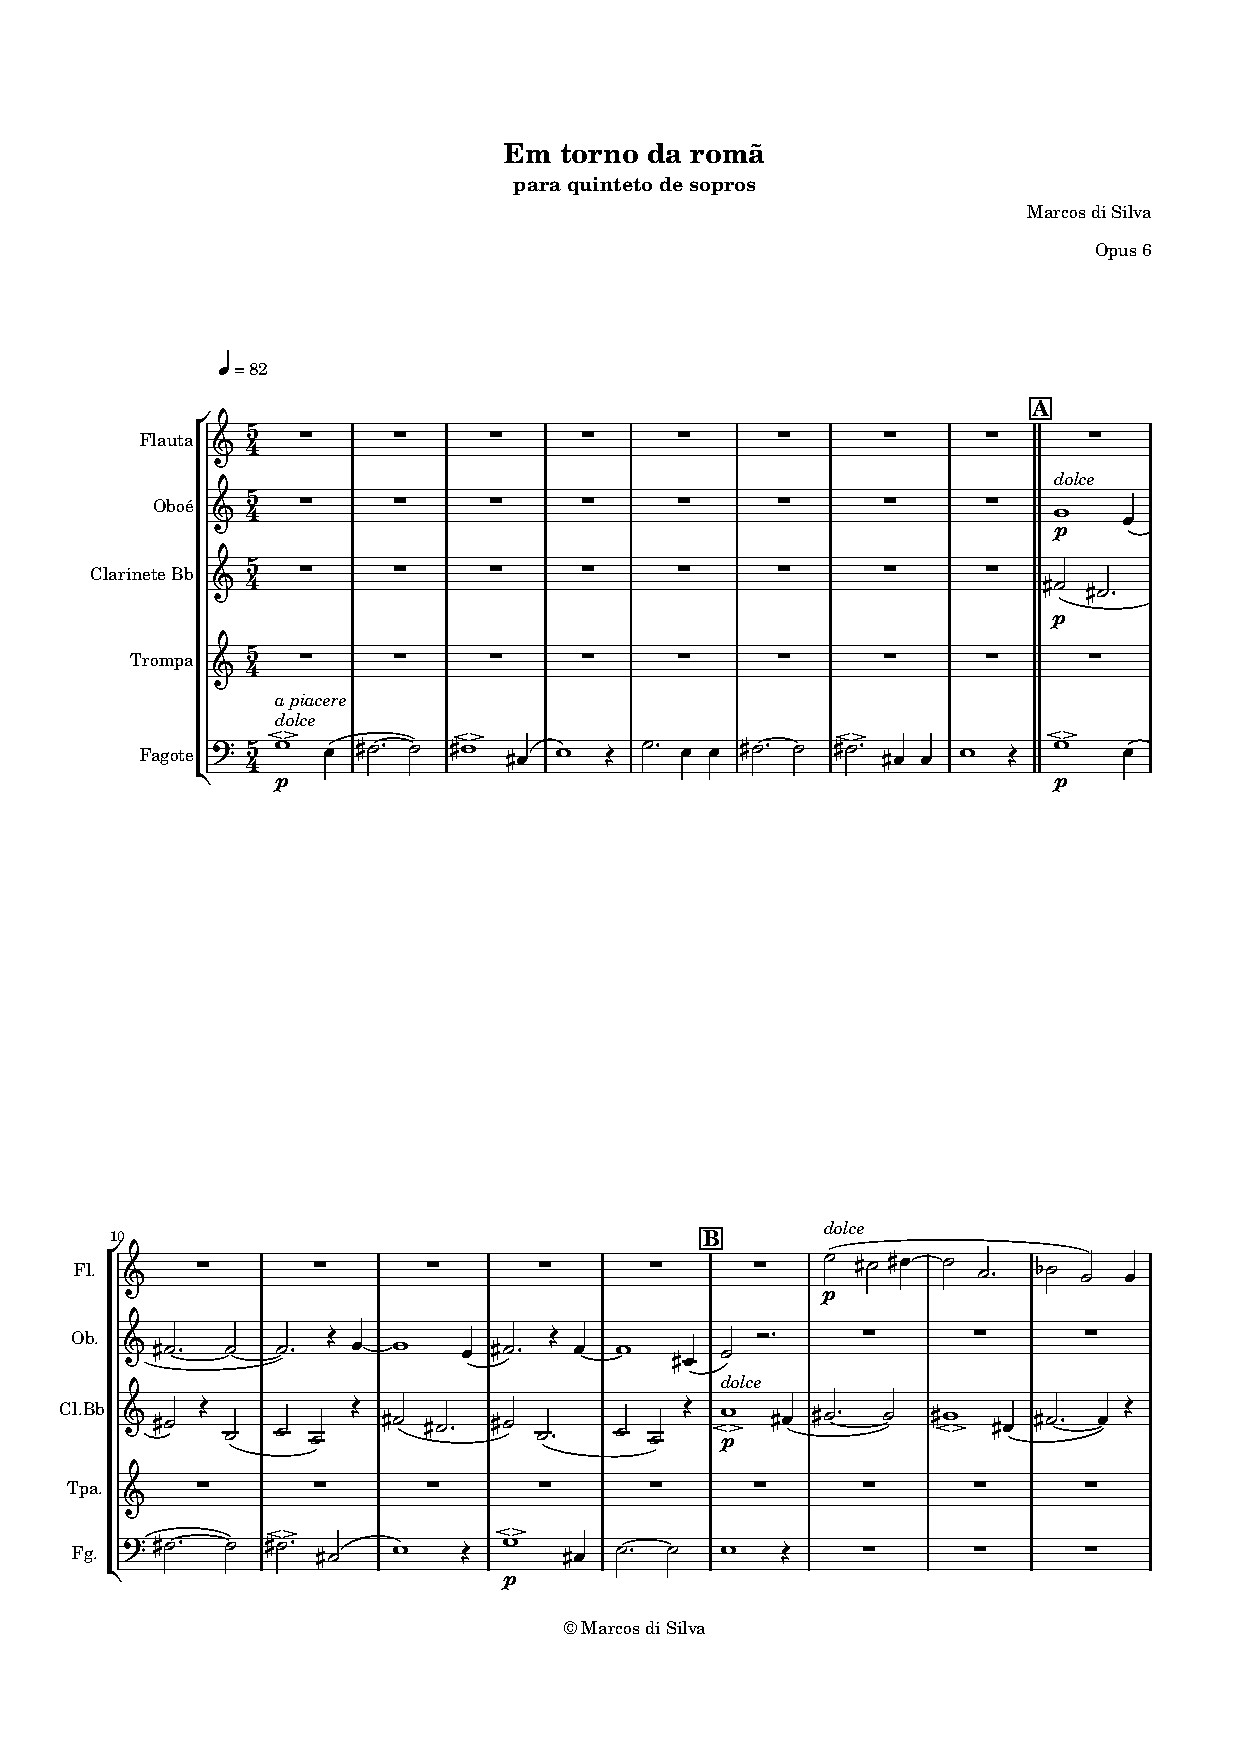
\includegraphics[scale=.55]{pagina-inicial-opus-6}
}

\frame{
  \frametitle{Materiais utilizados}
  \vspace{-2em}
  \begin{columns}[t]
    \hspace{-2em}
    \column[T]{5cm}
    \begin{figure}
      \centering
      \includegraphics[scale=1]{bifonia}
      \vspace{-2em}
      \caption{Estrutura de duas vozes}
    \end{figure}

    \vspace{-4em}
    \begin{figure}
      \centering
      \includegraphics[scale=1]{motivo-alfa}
      \vspace{-2em}
      \caption{Motivo $\alpha$}
    \end{figure}

    \column{4cm}
    \begin{figure}
      \centering
      \includegraphics[scale=1]{c-534120}
      \caption{Contorno P(5 3 4 1 2 0)}
    \end{figure}
  \end{columns}
}

\frame{
  \frametitle{Planejamento da composição}
  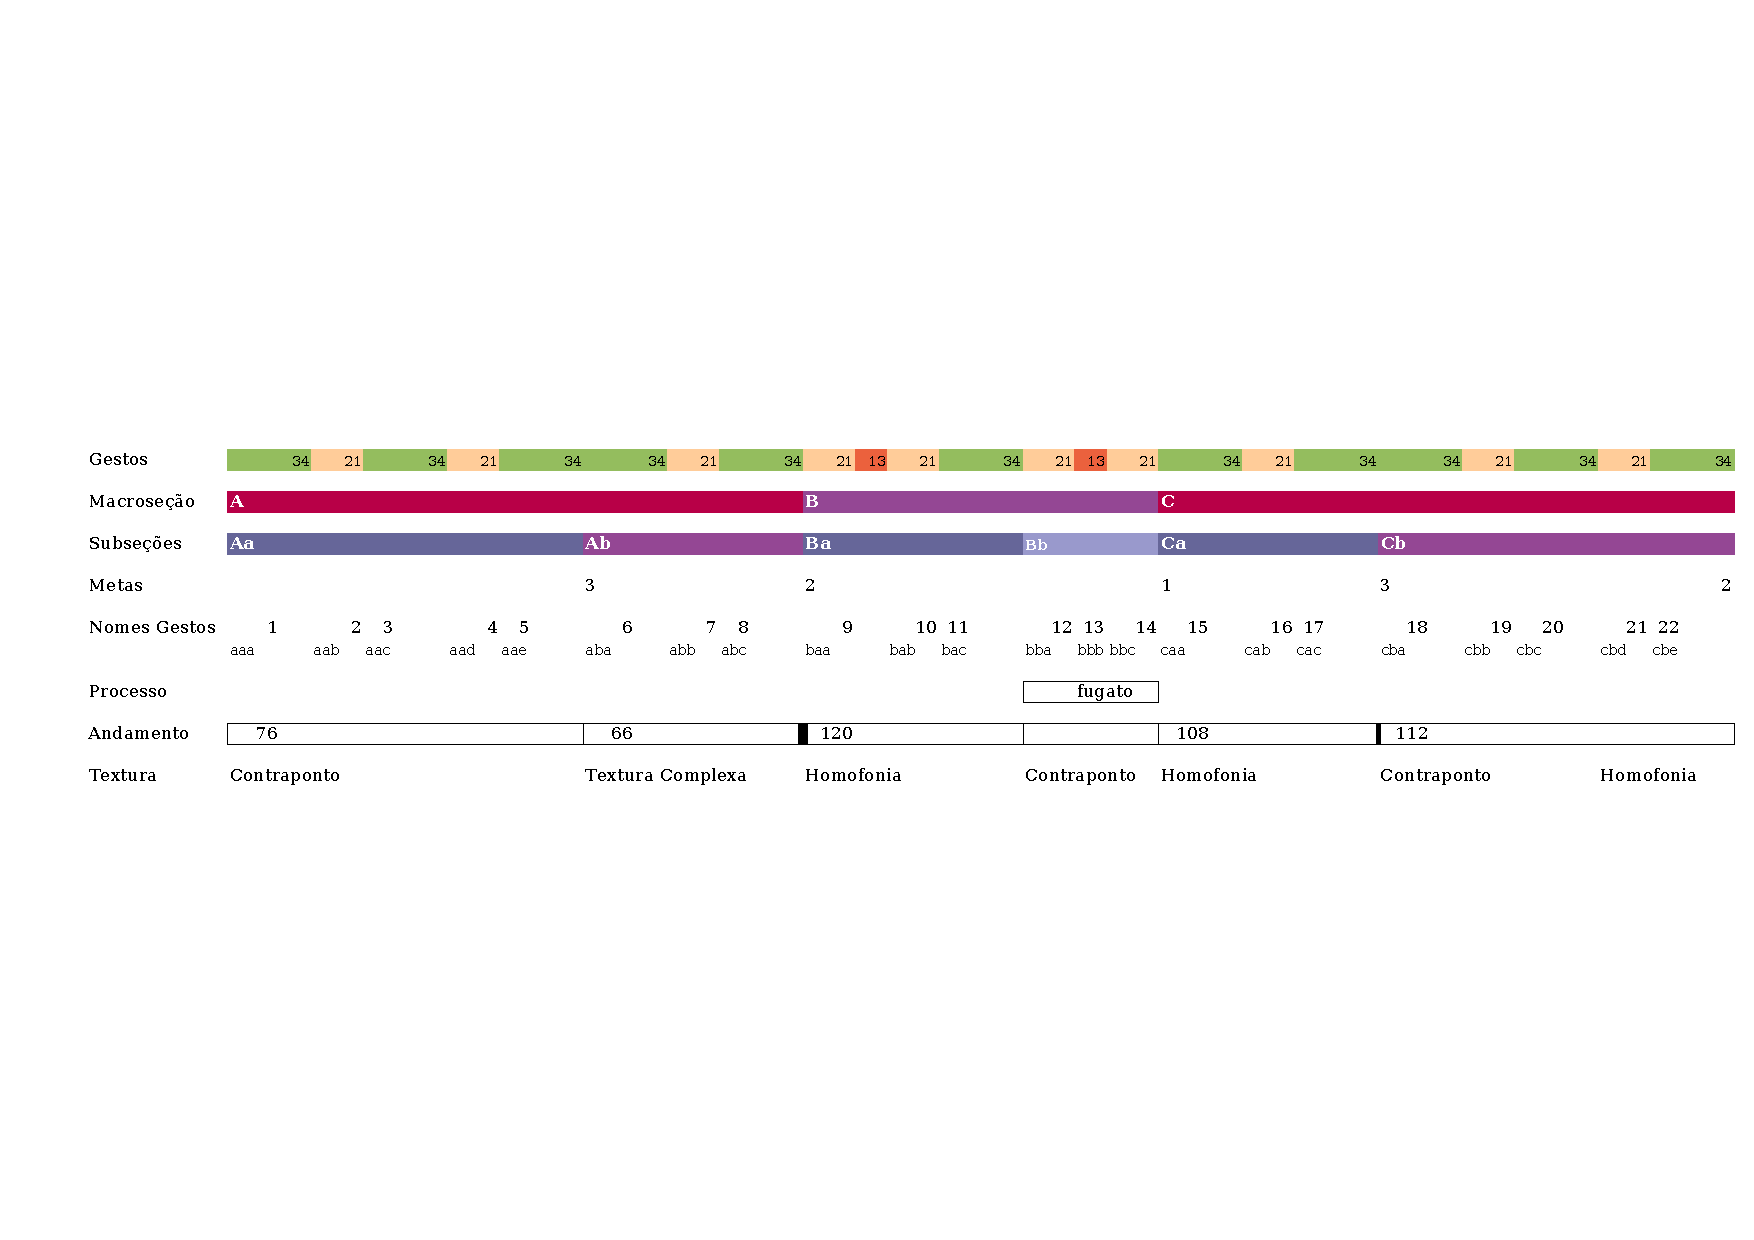
\includegraphics[scale=.4]{planejamento-inicial}
}

\frame{
  \frametitle{Descrição das seções}
  (ver na partitura)
}

\frame{
  \frametitle{Aspectos verticais}
  \begin{columns}[t]
    \column[T]{6cm}
    \begin{figure}
      \centering
      \includegraphics[scale=1]{bifonia}
      \vspace{-2em}
      \caption{Estrutura de duas vozes}
    \end{figure}

    \vspace{-5em}
    \begin{figure}
      \centering
      \includegraphics[scale=1]{escala-octatonica}
      \vspace{-2em}
      \caption{Escala octatônica}
    \end{figure}

    \column{6cm}
    \begin{figure}
      \centering
      \includegraphics[scale=1]{acorde-motivo}
      \vspace{-2em}
      \caption{Acorde motivo}
    \end{figure}
  \end{columns}
}

\frame{
  \frametitle{Uso de motivos}
  \vspace{-4em}
  \begin{columns}
    \hspace{-3em}
    \column{5cm}
    \begin{figure}
      \includegraphics[scale=1]{motivo-alfa-analisado}
      \vspace{-2em}
      \caption{Estrutura do motivo $\alpha$}
    \end{figure}
    \vspace{-4em}
    \begin{figure}
      \includegraphics[scale=.85]{motivo-delta}
      \vspace{-2em}
      \caption{Motivo $\delta$}
    \end{figure}

    \column{4cm}
    \begin{figure}
      \includegraphics[scale=1]{motivo-gama}
      \vspace{-2em}
      \caption{Motivo $\gamma$}
    \end{figure}
    \vspace{-4em}
    \begin{figure}
      \includegraphics[scale=1]{motivo-beta}
      \vspace{-2em}
      \caption{Motivo $\beta$}
    \end{figure}
  \end{columns}
}

\frame{
  \frametitle{Motivos $\alpha$ e $\beta$}
  \hspace{-2em} \includegraphics[scale=.7]{lily-044813d1e9-4}
}

\frame{
  \frametitle{Motivo $\gamma$}
  \hspace{-2em} \includegraphics[scale=.7]{lily-044813d1e9-29}
}

\frame{
  \frametitle{Motivo $\delta$}
  \hspace{-2em} \includegraphics[scale=.7]{lily-044813d1e9-14}
}

\frame{
  \frametitle{Contorno principal}
  \begin{figure}
    \centering
    \includegraphics[scale=1]{c-534120}
    \caption{Contorno P(5 3 4 1 2 0)}
  \end{figure}
}

\frame{
  \frametitle{Subconjunto de contorno com expansão e transposição}
  \begin{figure}
    \centering
    \includegraphics[scale=1]{melodia-inicial}

    \includegraphics{c-201}
  \end{figure}
}

\frame{
  \frametitle{Interpolação com expansão}
  \begin{figure}
    \centering
    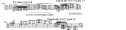
\includegraphics[scale=4.8]{oboe-solo-secao-5}
  \end{figure}
}

\frame{
  \frametitle{Rotação com expansão}
  \begin{figure}
    \centering
    \includegraphics[scale=.7]{notas-curtas-madeiras}

    \includegraphics[scale=.55]{c-534120}
    \includegraphics[scale=.55]{c-412053}
    \includegraphics[scale=.55]{c-120534}
    \includegraphics[scale=.55]{c-435021}
  \end{figure}
}

\frame{
  \frametitle{Rotação com retrogradação}
  \begin{figure}
    \centering
    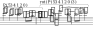
\includegraphics[scale=2.5]{sujeito-fugato}

    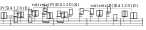
\includegraphics[scale=2.5]{contra-sujeito-fugato}
  \end{figure}
}

\frame{
  \frametitle{Int$_1$}
  (- + - + -)

  \hspace{-2em} \includegraphics[scale=.7]{lily-044813d1e9-29}
}

\frame{
  \frametitle{Expansão associada à amplitude}
  \begin{figure}
    \centering
    \includegraphics[scale=.8]{escala-secao-2-one}
  \end{figure}
}

\frame{
  \frametitle{Expansão associada à amplitude}
  \begin{figure}
    \centering
    \includegraphics[scale=.6]{secao-2}
  \end{figure}
}

\frame{
  \frametitle{Redução de contornos}
  \begin{figure}
    \centering
    \includegraphics[scale=.8]{reducao-contornos-secao-3-clarinete}

    \includegraphics[scale=.8]{reducao-contornos-secao-3-oboe}

    \includegraphics[scale=.8]{reducao-contornos-secao-3-clarinete-2}
  \end{figure}
}

\frame{
  \frametitle{Contornos e outros parâmetros}
  \begin{itemize}
  \item Andamentos: 82, 66, 120, 108 e 112. A(1 0 4 2 3)
  \item Densidade. Seção 1: D(1 3 2 5 4)
  \item Complexidade de texturas: (- + - + -)
  \end{itemize}
}

\section{Conclusões}

\frame{
  \frametitle{Conclusões}
  \begin{itemize}
  \item Discussão
  \item Trabalhos futuros
  \end{itemize}
}

\frame[allowframebreaks]{
  \frametitle{Referências}
  \bibliographystyle{alpha}
  \bibliography{melodic-contour,music-perception,composition,music-harmony-and-theory,programs,music-analysis,audio,genos,computer-science}
}

\end{document}
